\documentclass[a4paper,10pt]{IEEEtran}
\usepackage{mathptmx}

\usepackage{tabularx} % extra features for tabular environment
\usepackage{amsmath}  % improve math presentation
\usepackage{float}
% \usepackage{pdfpages}


\usepackage{graphicx} % takes care of graphic including machinery
\graphicspath{ {./figures/} }
%\usepackage[margin=1in,letterpaper]{geometry} % decreases margins
%\usepackage{cite} % takes care of citations
\usepackage[final]{hyperref} % adds hyper links inside the generated pdf file
\hypersetup{
	colorlinks=true,       % false: boxed links; true: colored links
	linkcolor=blue,        % color of internal links
	citecolor=blue,        % color of links to bibliography
	filecolor=magenta,     % color of file links
	urlcolor =blue         
}
\usepackage[margin = 1in,headsep=0.5cm,headheight=2cm,letterpaper]{geometry} 

\usepackage{fancyhdr}
\pagestyle{fancy}
\lhead{Student 1 : Ahmet Akman 2442366 \\ Student 2: Kaan Demirkoparan }
\rhead{Date: \today \\ Group: Friday Morning - 6} 
%\cfoot{center of the footer!}
%\renewcommand{\headrulewidth}{0.1pt}


\begin{document}
%\thispagestyle{empty}

\title{  Fall 2022 EE Project Work  \protect\\ Preliminary Report}
\author{ Ahmet Akman 2442366 \protect\\ Kaan Demirkoparan}
\date{}
\maketitle
%\tableofcontents
%\begin{abstract}
%abstract
%\end{abstract}
\section{Introduction}
In this document, the Preliminary report of the term project of the EE214 course will be presented. 
\section{General Structure and Design Philisophy}
\begin{figure}[h]
    \centering
    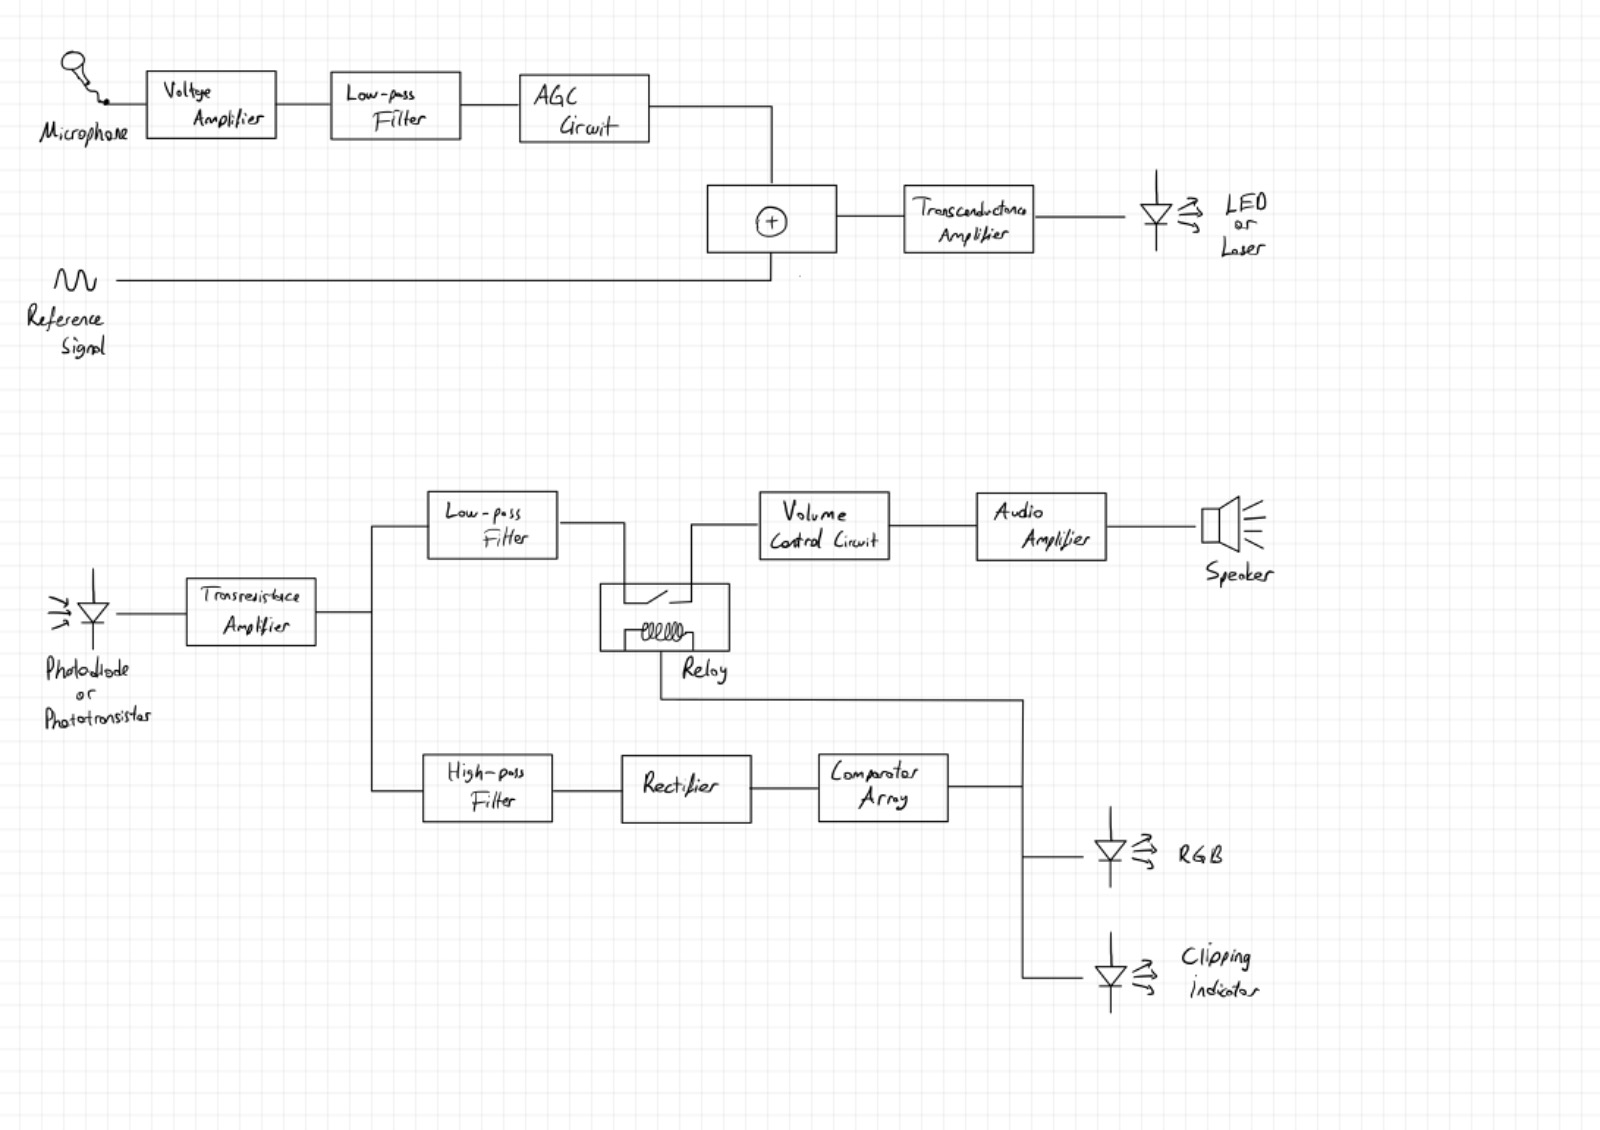
\includegraphics[width = 1\linewidth]{general_structure.jpeg}
    \caption{General Structure}
\end{figure} 
Deneme
Deneme 123 Deneme 123

xyz

\section{Transmitter Side}
\subsection{Input and Early Stage Amplification}
\subsection{Automatic Gain Control}
\subsection{Light Transmitter}
\section{Receiver Side}
\subsection{Light Receiver}
\subsection{Demodulation and Speaker Side}
At the beggining of this stage a simple op-amp buffer will planned to be used in order to prevent distorion while using the same signal as input for two stages in parallel. For the demodulation of the input signal (a.k.a. filtering out the carrier high frequency components), a low pass filter will planned to be used. There are two basic  option for low pass filtering. First one is passive RC/RL filters. They use few components but have no gain and there is no tunability. Second one is active opamp-filters. Even though they seem more complicated one can have gain and a more flexible design. The required low pass charachteristic is given in Figure \ref*{low_pass_plot}
\begin{figure}[H]
    \centering
    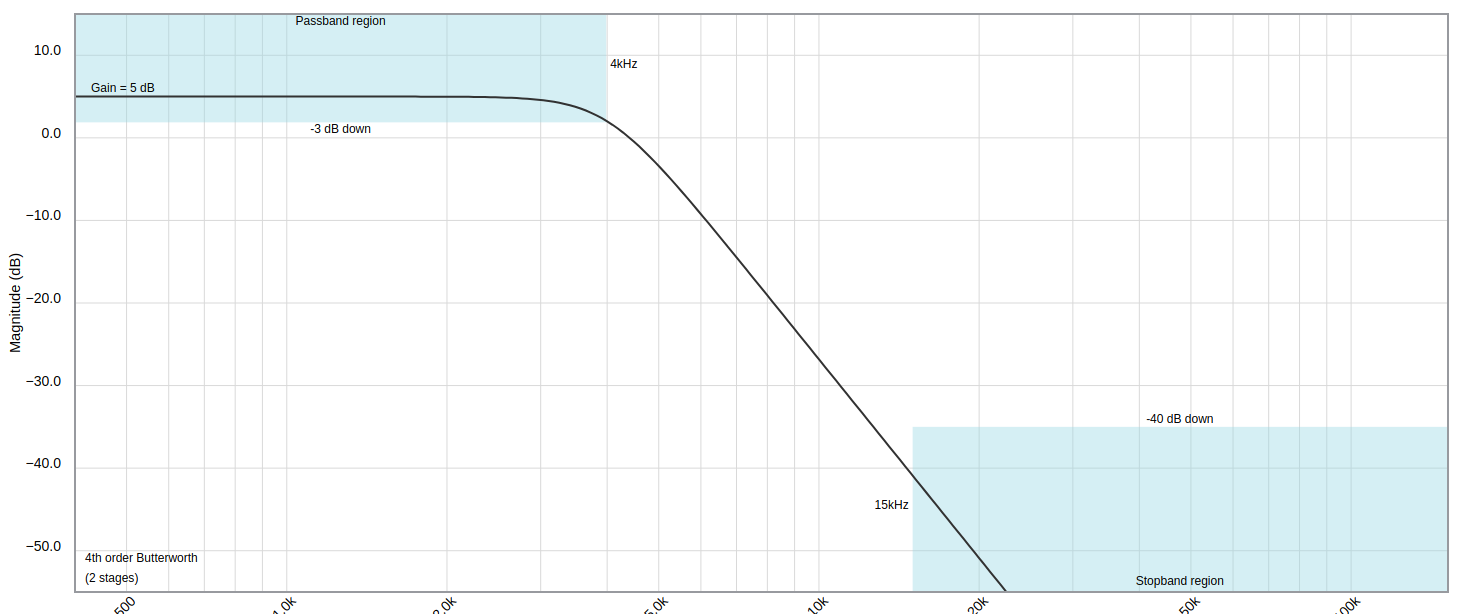
\includegraphics[width = 0.75\linewidth]{active_low_pass.png}
    \caption{Low pass filter frequency response}
    \label{low_pass_plot}    
\end{figure} 
Because of the aforementioned advantages our design decision is using active two stage low pass filter with butterworth response charachteristic. A premature design is given in Figure \ref*{low_pass_sch}
\begin{figure}[H]
    \centering
    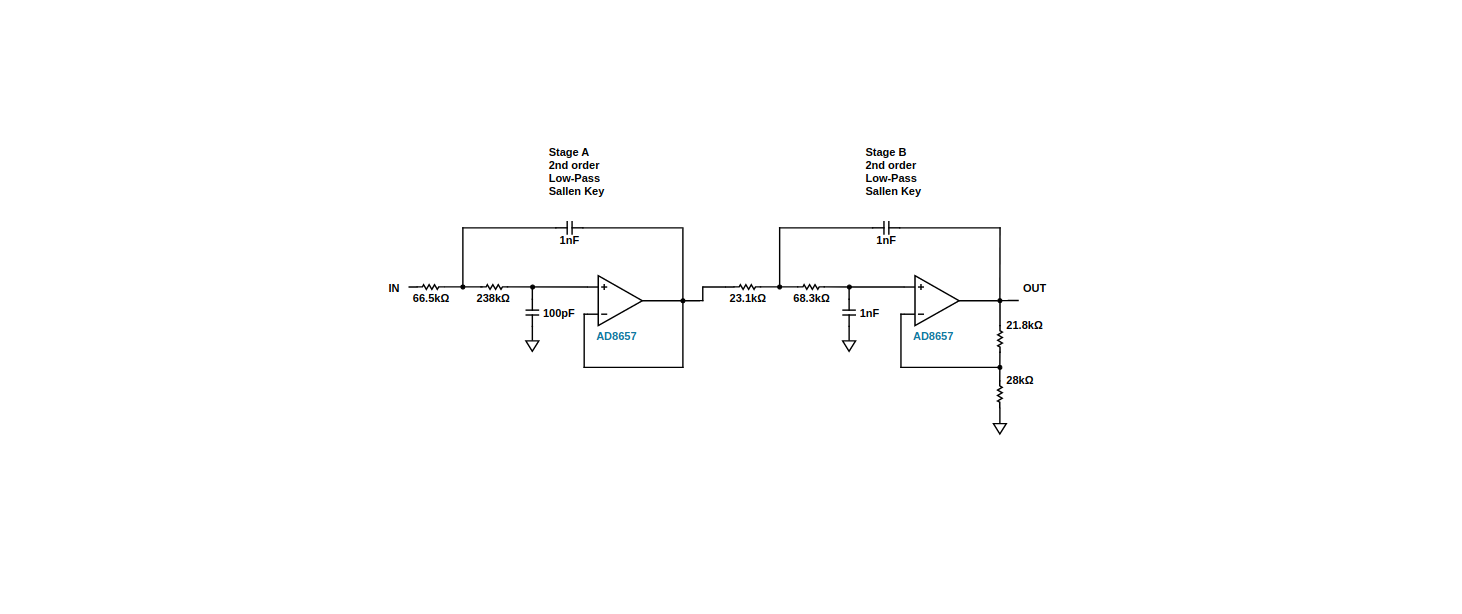
\includegraphics[width = 0.75\linewidth]{active_low_pass_circuit.png}
    \caption{Active low pass filter design}
    \label{low_pass_sch}    
\end{figure} 
\subsubsection{Low Signal Switch and Saturation Indicator}
%LOW SİGNAL SWİTCH PART WILL BE ADDED
The requirements of the projects indicates that if there is a small signal below a threshold there should be no sound. On the other hand it is given that if there are a saturated signal a LED should indicate this situation. So, to adress both design problems design based on a voltage peak dedector is proposed. Peak dedector detects the peaks and the cascaded comparators compares the signal with reference dc values. To be able to adjust the threshold voltages voltage dividers are utilized. For the low amplitude cut off a mosfet switch is added afterwards. This stage of the design is given in Figure \ref*{saturated_ind} 
\begin{figure}[H]
    \centering
    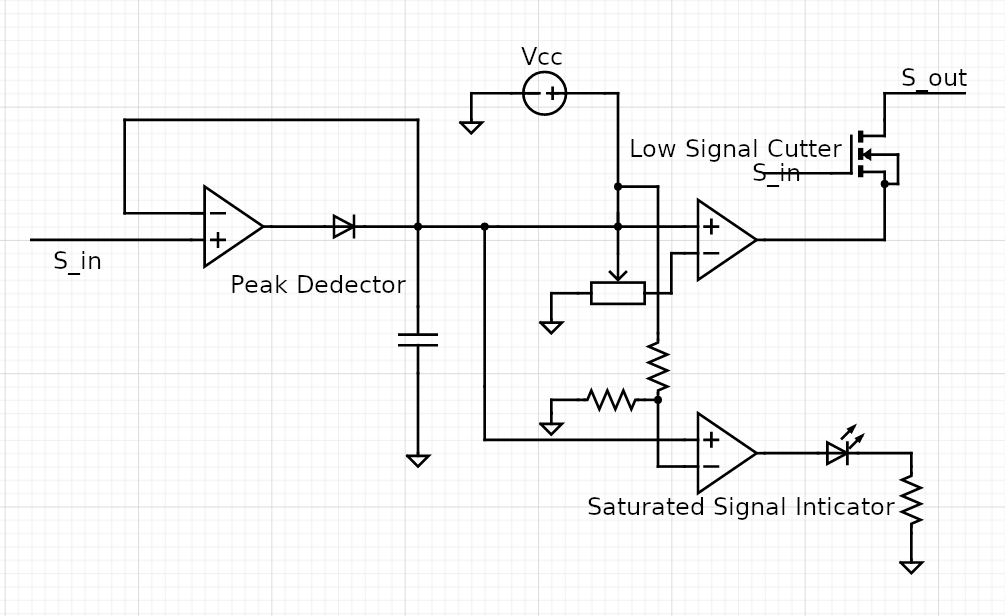
\includegraphics[width = 0.75\linewidth]{LowSignalSatSignal.png}
    \caption{Low and saturated signal switches.}
    \label{saturated_ind}    
\end{figure} 

\subsubsection{Volume Control}
In order to adjust manually the level of volume, very well known active volume control circuit called "Baxandall" will be used. The schematic of the block is given in Figure \ref*{Baxandall}. An opamp ic with 2 opamp such as TL072 or LM358 will be used as the amplifier in the schematic. 

\begin{figure}[H] %https://www.ti.com/lit/ug/tidu034/tidu034.pdf?ts=1672401791602&ref_url=https%253A%252F%252Fwww.google.com%252F
    \centering
    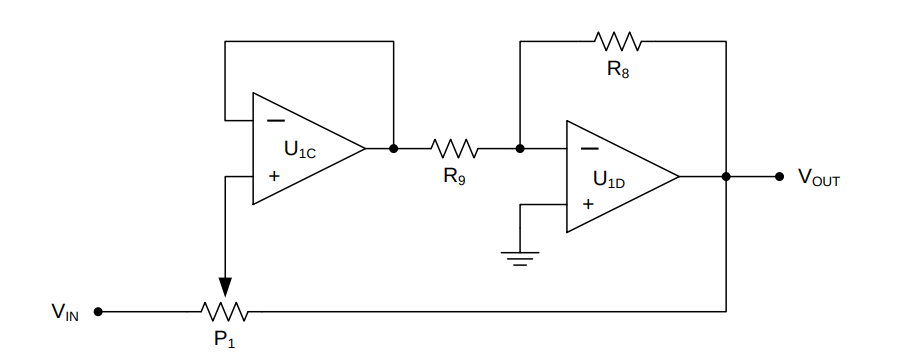
\includegraphics[width = 0.75\linewidth]{baxandall_volume_control.png}
    \caption{Active volume control circuit}
    \label{Baxandall}    
\end{figure} 
Since, now we have a nice signal that carries the information needed, we should amplify it properly in order to drive the speaker. For the design purpose we assume our speaker is 16\(\Omega\) ,and our design constraint is that our speaker will operate with 1W power. There are couple of options to drive speaker such as Class A, Class B, Class AB and Class C. For our driving purposes a Class AB amplifier is planned to be used because of low distorion and higher efficiency compared to class A and B amplifier topologies. A schematic for such a stage is given in Figure \ref*{power_amp_sch}.
\begin{figure}[H]
    \centering
    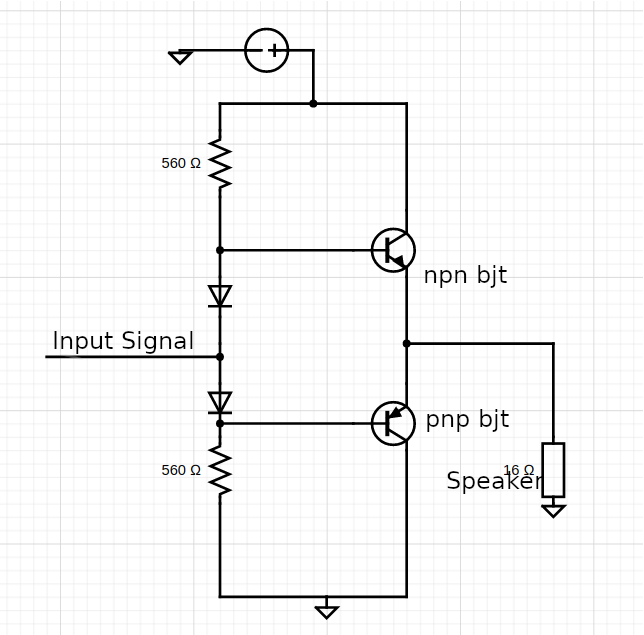
\includegraphics[width = 0.75\linewidth]{power_amp.png}
    \caption{Power amplifier and speaker unit.}
    \label{power_amp_sch}    
\end{figure} 
   
\subsection{Signal Quality Indication}
One of the requirements of the project is an indication of the signal quality. To be able to extract the carrier signal from overall signal, an active high-pass filter with Chebyshev response. Similar to the low-pass case a buffer stage will be added before the filter. The design with two stages is shown in Figure \ref*{active_high}.
\begin{figure}[H]
    \centering
    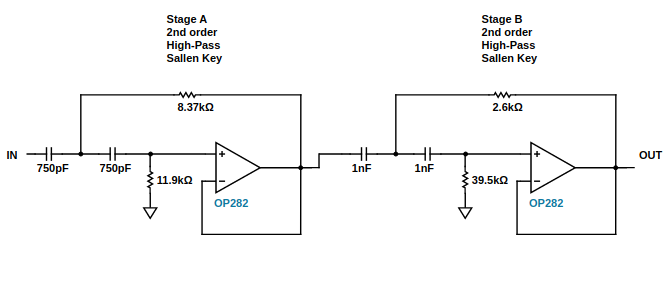
\includegraphics[width = 0.75\linewidth]{active_high_pass_circuit.png}
    \caption{Power amplifier and speaker unit.}
    \label{active_high}    
\end{figure} 

Again a simple peak dedector will be utilized in order to discriminate the signal quality level.The peak value of the reference signal is then compared to four different reference voltages. Based on the comparison, an RGB light will display different colors depending on the voltage level. The specific colors that will be displayed are determined by the comparison of the voltage to the reference voltages, with green being displayed if the voltage is less than or greater than a certain range, red being displayed if the voltage is above a certain level, and blue being displayed if the voltage is above another level. The goal of this process is to display different colors of the RGB light in different cases. The designed schematic is given in Figure \ref*{indicator}
\begin{figure}[H]
    \centering
    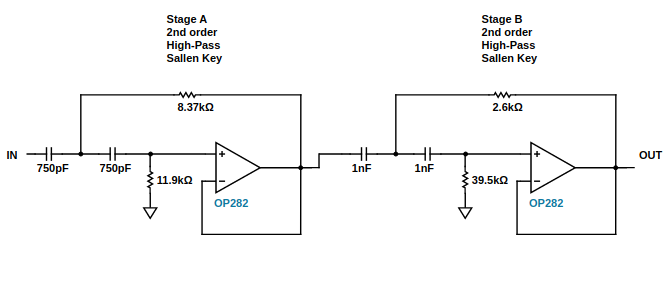
\includegraphics[width = 0.75\linewidth]{active_high_pass_circuit.png}
    \caption{Signal Level Indicator part}
    \label{indicator}    
\end{figure} 
\section{Conclusion}
In this document, the Preliminary report of the term project of the EE313 course is presented. 

\end{document}

%%%%%%%%%%%%%%%%%%%%%%   EXAMPLE TABLE   %%%%%%%%%%%%%%%%%%%%%%%%%%%%%%%%
\begin{table}[H]
\begin{center}
    \caption{Resistance reading by color code convention.}
    \vspace{2mm}
    \begin{tabular}{||c | c | c||} 
        \hline
        Color Order & Value & Tolerance \\ [0.5ex] 
        \hline\hline
        Brown / Black / Red / Gold & 1k\( \Omega \) & \( \% \) 5  \\ 
        \hline
        Yellow / Violet / Red / Gold & 4.7k\( \Omega \) & \( \% \) 5   \\
        \hline
        Brown / Grey / Orange / Gold & 18k\( \Omega \) & \( \% \) 5  \\ [1ex] 
        \hline
    \end{tabular}
\end{center}
\end{table}


%%%%%%%%%%%%%%%%%%%%%%   EXAMPLE IMAGE   %%%%%%%%%%%%%%%%%%%%%%%%%%%%%%%%
\begin{figure}[H]
\centering
\includegraphics[width = 0.75\textwidth]{5.png}
\caption{Circuit schematic for the step 5}
\end{figure} 

%%%%%%%%%%%%%%%%%%%%%%   EXAMPLE IMAGE FROM PDF   %%%%%%%%%%%%%%%%%%%%%%%%%%%%%%%%
\begin{figure}[H] \centering{
	\includegraphics[scale=0.25]{2a_plot.pdf}}
	\caption{Experiment 2}
\end{figure}
%%%%%%%%%%%%%%%% Deneme Push